\documentclass{beamer}
%\usetheme{Darmstadt}
\setbeamertemplate{navigation symbols}{}
\setbeamertemplate{footline}[page number]
\usefonttheme{professionalfonts}
\usepackage{comment}
\usepackage{xcolor}
\usepackage{colortbl} % Needed for \rowcolor
%\usepackage[%
%style=authoryear,
%doi=false,
%isbn=false,
%url=false,
%eprint=false]{bibtex}
%\usepackage[backend=biber]{biblatex}
%\addbibresource{references.bib}
\usepackage{setspace}
\usepackage{bbm}

\definecolor{navy}{RGB}{0,0,128}

\title{Dirichlet-Multinomial Supplement}
\author{Gwen Jacobson}
\institute[]{Duke University}

\newcommand{\indep}{\perp \!\!\! \perp}

\begin{document}
\bibliographystyle{plainnat}
\frame[plain,noframenumbering]{\titlepage}

\begin{frame}{Overview}
    \begin{itemize}
        \item Simplex Review
        \item Dirichlet Distribution
        \item Categorical Distribution
        \item Multinomial Distribution
        \item Bayesian Inference
        \item Properties and Sampling Proofs
    \end{itemize}
\end{frame}

\begin{frame}{Review: The Simplex}
The $(K-1)$-\textbf{dimensional simplex} $\Delta^{K - 1}$ is the subspace of $\mathbb{R}^{K}$ on which $K$-component probability vectors live. That is, $$\Delta^{K - 1} = \left\{\left(\pi_{1},\dots, \pi_{K}\right) \in \mathbb{R}^{K}:~\pi_{k} \geq 0, \sum_{k = 1}^{K}{\pi_{k}} = 1\right\}.$$ ``$(K - 1)$-dimensional" means that, once you have $(K - 1)$ components of the vector, there are no more free components.
\begin{figure}[htbp]
\begin{center}
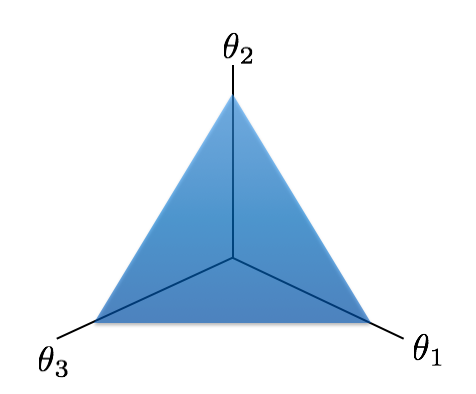
\includegraphics[width=0.3\textwidth]{figures/simplex.png}
\caption{The two-dimensional simplex in $\mathbb{R}^{3}$.}
\end{center}
\end{figure}
\end{frame}

\begin{frame}{The Dirichlet Distribution}
\only<1>{The $K$\textbf{-component Dirichlet distribution} is a probability distribution over the $(K - 1)$-dimensional simplex. It is a generalization of the Beta distribution.

\vspace{10pt}

It may be parameterized by a vector $\boldsymbol{\alpha} = \left(\alpha_{1},\dots,\alpha_{K}\right)$, $\alpha_{k} > 0$, of concentration parameters. 

\vspace{10pt}

We then say $$\boldsymbol{\pi} = \left(\pi_{1},\dots,\pi_{K}\right) \sim \text{Dirichlet}(\boldsymbol{\alpha})$$ if $$p\left(\pi_{1},\dots, \pi_{K}\right) = \frac{\Gamma\left(\sum_{k = 1}^{K}{\alpha_{k}}\right)}{\prod_{k = 1}^{K}{\Gamma\left(\alpha_{k}\right)}}\prod_{k = 1}^{K}{\pi_{k}^{\alpha_{k} - 1}} \cdot \mathbbm{1}\left[\boldsymbol{\pi} \in \Delta^{K - 1}\right].$$
}
\only<2>{The Dirichlet may also be parameterized by a single concentration scalar $\alpha > 0$ and its mean vector $\boldsymbol{\nu} \in \Delta^{K - 1}$, where $\boldsymbol{\alpha} = \alpha\boldsymbol{\nu}$.

\vspace{10pt}

To recover $\alpha$ and $\boldsymbol{\nu}$ from $\boldsymbol{\alpha}$, we normalize $\boldsymbol{\alpha}$ by the sum of its components (the $1$-norm $||\boldsymbol{\alpha}||_{1} = \sum_{k = 1}^{K}{\left|\alpha_{k}\right|}$), getting $$\alpha = ||\boldsymbol{\alpha}||_{1} \qquad \boldsymbol{\nu} = \frac{\boldsymbol{\alpha}}{||\boldsymbol{\alpha}||_{1}} = \left(\frac{\alpha_{1}}{\sum_{k = 1}^{K}{\alpha_{k}}}, \dots, \frac{\alpha_{K}}{\sum_{k = 1}^{K}{\alpha_{k}}}\right).$$ Verify for yourself that $\boldsymbol{\nu} \in \Delta^{K - 1}$.
}

\only<3>{
When doing mathematical calculations with the Dirichlet density, one of the $\pi_{k}$ -- say, $\pi_{K}$ -- must be the ``non-free" variable. That is, $$p\left(\pi_{1},\dots, \pi_{K}\right) = \frac{\Gamma\left(\sum_{k = 1}^{K}{\alpha_{k}}\right)}{\prod_{k = 1}^{K}{\Gamma\left(\alpha_{k}\right)}}\prod_{k = 1}^{K}{\pi_{k}^{\alpha_{k} - 1}} \cdot \mathbbm{1}\left[\boldsymbol{\pi} \in \Delta^{K - 1}\right],$$ where $\pi_{K}$ is a more compact way of writing $1 - \sum_{k = 1}^{K - 1}{\pi_{k}}$. 

\vspace{10pt}

For the two-component Dirichlet, $$p\left(\pi_{1}, \pi_{2}\right) = \frac{\Gamma\left(\alpha_{1} + \alpha_{2}\right)}{\Gamma\left(\alpha_{1}\right)\Gamma\left(\alpha_{2}\right)}\pi_{1}^{\alpha_{1} - 1}\pi_{2}^{\alpha_{2} - 1} \cdot \mathbbm{1}\left[\boldsymbol{\pi} \in \Delta^{1}\right].$$ Since there is only one free variable (pick $\pi_{1}$), this collapses to the univariate $$p\left(\pi_{1}\right) = \frac{\Gamma\left(\alpha_{1} + \alpha_{2}\right)}{\Gamma\left(\alpha_{1}\right)\Gamma\left(\alpha_{2}\right)}\pi_{1}^{\alpha_{1} - 1}\left(1 - \pi_{1}\right)^{\alpha_{2} - 1} \cdot \mathbbm{1}\left[\pi_{1} \in [0, 1]\right],$$ which is the $\text{Beta}\left(\alpha_{1}, \alpha_{2}\right)$ distribution.
}
\end{frame}

\begin{frame}{Dirichlet Mean}
If $\boldsymbol{\pi} \sim \text{Dirichlet}(\boldsymbol{\alpha})$ with concentration $\alpha = ||\boldsymbol{\alpha}||_{1}$ and mean vector $\boldsymbol{\nu}$, we have that 
\begin{align*}
\mathbb{E}[\boldsymbol{\pi}] = \boldsymbol{\nu} & = \left(\frac{\alpha_{1}}{||\boldsymbol{\alpha}||_{1}},\dots, \frac{\alpha_{K}}{||\boldsymbol{\alpha}||_{1}}\right) \\ & = \left(\frac{\alpha_{1}}{\sum_{k = 1}^{K}{\alpha_{K}}},\dots, \frac{\alpha_{K}}{\sum_{k = 1}^{K}{\alpha_{K}}}\right) \\ & = \left(\mathbb{E}\left[\pi_{1}\right],\dots,\mathbb{E}\left[\pi_{K}\right]\right).
\end{align*}
$\boldsymbol{\nu}$ determines the location of the center of mass for the density, while $\alpha$ determines the direction and spread of the mass. 
\begin{itemize}
    \item $0 < \alpha < 1$: diffuse away from $\boldsymbol{\nu}$
    \item $\alpha = 1$: uniform
    \item $\alpha > 0$: concentrated toward $\boldsymbol{\nu}$
\end{itemize}
\end{frame}

\begin{frame}{Examples}
\only<1>{
\begin{figure}[htbp]
\begin{center}
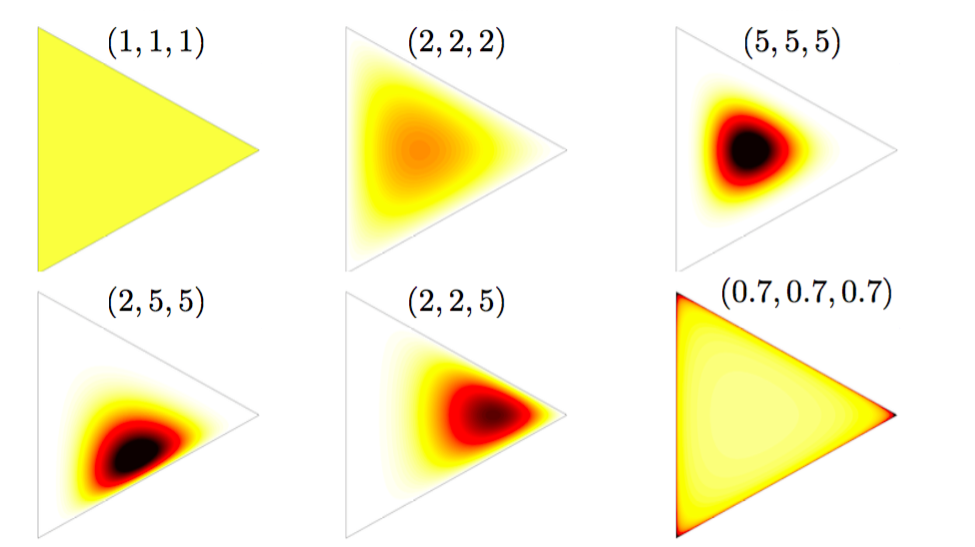
\includegraphics[width=0.9\textwidth]{figures/dir}
\caption{Top row: Mean at the centroid of the simplex, starting with uniform and getting more concentrated. Bottom row: Two concentrated and centered away from the centroid, and one centered at the centroid but diffuse to the vertices.}
\label{default}
\end{center}
\end{figure}}
\only<2>{
See DirichletDistributions.pdf (kindly provided by Mark Jacobson) in the Lecture 7 figures repository for non-heatmap example Dirichlet densities.
}
\end{frame}

\begin{frame}{The Categorical Distribution}
    Suppose $X$ can belong to one of $K$ distinct categories, with the probability of belonging to category $k$ equal to $$\mathbb{P}(X = k) = \pi_{k}.$$ We say that $X$ follows a \textbf{Categorical distribution}, parameterized by a $K$-component probability vector $\boldsymbol{\pi} \in \Delta^{K - 1}$. We can alternatively express the PMF as $$p(x) = \prod_{k = 1}^{K}{\pi_{k}^{\mathbbm{1}[x = k]}} \cdot \mathbbm{1}[x \in \{1,\dots, K\}].$$ 
\end{frame}

\begin{frame}{The Multinomial Distribution}
    \only<1>{Suppose you have $n$ i.i.d. $\text{Categorical}(\boldsymbol{\pi})$ draws and consider the distribution of their category counts $\mathbf{Y} = \left(Y_{1},\dots, Y_{K}\right)$. 
    
    \vspace{10pt}
    
    This vector of counts follows a \textbf{Multinomial distribution}, which is a multivariate generalization to the Binomial distribution.

    \vspace{10pt}

    Let $\mathbf{y} = \left(y_{1},\dots, y_{K}\right)$. We say that $$\mathbf{Y} = \left(Y_{1},\dots, Y_{K}\right) \sim \text{Multinomial}(n, \boldsymbol{\pi})$$ if $$\mathbb{P}(\mathbf{Y} = \mathbf{y} \mid \boldsymbol{\pi}) = \binom{n}{y_{1}\cdots y_{K}}\prod_{k = 1}^{K}{\pi_{k}^{y_{k}}} \cdot \mathbbm{1}\left[\sum_{k = 1}^{K}{y_{k}} = n\right],$$ where $\binom{n}{y_{1}\cdots y_{K}}$ is the \textit{multinomial coefficient} such that $$\binom{n}{y_{1}\cdots y_{K}} = \frac{n!}{\prod_{k = 1}^{K}{y_{k}!}}.$$}
    \only<2>{
    As with the Dirichlet distribution, one of the $Y_{k}$ -- say, $Y_{K}$ -- is not free. That is, $$\mathbb{P}(\mathbf{Y} = \mathbf{y}) = \binom{n}{y_{1}\cdots y_{K}}\prod_{k = 1}^{K}{\pi_{k}^{y_{k}}} \cdot \mathbbm{1}\left[\sum_{k = 1}^{K}{y_{k}} = n\right],$$ where $y_{K}$ is a compact way of writing $n - \sum_{k = 1}^{K - 1}{y_{k}}$.

    \vspace{10pt}

    For the two-component Multinomial, $$\mathbb{P}(\mathbf{Y} = \mathbf{y}) = \binom{n}{y_{1} \; \; \; y_{2}}\pi_{1}^{y_{1}}\pi_{2}^{y_{2}} \cdot \mathbbm{1}\left[y_{1} + y_{2} = n\right].$$ Pick $y_{1}$ as the free component; note that, since $\boldsymbol{\pi} \in \Delta^{1}$, we can also rewrite $\pi_{2}$ in terms of $\pi_{1}$. So, this collapses to the univariate $$\mathbb{P}\left(Y_{1} = y_{1}\right) = \binom{n}{y_{1}}\pi_{1}^{y_{1}}\left(1 - \pi_{1}\right)^{n - y_{1}} \cdot \mathbbm{1}\left[y_{1} \in \{0,\dots, n\}\right],$$ which is the $\text{Binomial}\left(n, \pi_{1}\right)$ distribution.  
    }
\end{frame}

\begin{frame}{Posterior Updating}
    \only<1>{Suppose you have the following Bayesian model:
    \begin{align*}
        \mathbf{Y} \mid \boldsymbol{\pi} & \sim \text{Multinomial}(n, \boldsymbol{\pi}) \\ \boldsymbol{\pi} & \sim \text{Dirichlet}(\boldsymbol{\alpha}).
    \end{align*}
    Just as the Beta distribution is a conjugate prior to the Binomial likelihood, the Dirichlet is a conjugate prior to the Multinomial likelihood.}
    \only<2>{
    The posterior updating proceeds as follows:
    \begin{align*}
        p\left(\boldsymbol{\pi} \mid \mathbf{Y}\right) & \propto p(\mathbf{Y} \mid \boldsymbol{\pi}) \times p(\boldsymbol{\pi}) \\ & \propto \left(\binom{n}{y_{1}\cdots y_{K}}\prod_{k = 1}^{K}{\pi_{k}^{y_{k}}}\right) \times \left(\frac{\Gamma\left(\sum_{k = 1}^{K}{\alpha_{k}}\right)}{\prod_{k = 1}^{K}{\Gamma\left(\alpha_{k}\right)}}\prod_{k = 1}^{K}{\pi_{k}^{\alpha_{k} - 1}}\right) \\ & \propto \left(\prod_{k = 1}^{K}{\pi_{k}^{y_{k}}}\right) \times \left(\prod_{k = 1}^{K}{\pi_{k}^{\alpha_{k} - 1}}\right) \\ & \propto \prod_{k = 1}^{K}{\pi_{k}^{\left(\alpha_{k}+ y_{k}\right) - 1}}.
    \end{align*}
    The posterior then has the form $$\boldsymbol{\pi} \mid \mathbf{Y} \sim \text{Dirichlet}(\boldsymbol{\alpha} + \mathbf{Y}).$$
    }
    \only<3>{
    Alternatively, we could deal with the Categorical likelihood, where $$X_{1},\dots, X_{n} \stackrel{\text{i.i.d.}}{\sim} \text{Categorical}(\boldsymbol{\pi}).$$ We then have the following:
    \begin{align*}
        p(\mathbf{x}) & = \prod_{i = 1}^{n}{p\left(x_{i}\right)} \\ & = \prod_{i = 1}^{n}{\prod_{k = 1}^{K}{\pi_{k}^{\mathbbm{1}\left[x_{i} = k\right]}}} \\ & = \prod_{k = 1}^{K}{\pi_{k}^{\sum_{i = 1}^{n}{\mathbbm{1}\left[x_{i} = k\right]}}}.
    \end{align*}
    If we set $y_{i} = \sum_{i = 1}^{n}{\mathbbm{1}\left[x_{i} = k\right]}$, we see that $$p(\mathbf{x}) = p(\mathbf{y}) = \prod_{k = 1}^{K}{\pi_{k}^{y_{i}}}$$ recovers (up to proportionality) the Multinomial likelihood.
    }
\end{frame}

\begin{frame}{Interpreting Prior Parameters}
    \only<1>{Recall that, with the $\text{Beta}\left(\alpha_{1}, \alpha_{2}\right)$ distribution, we identified
    \begin{itemize}
        \item $\alpha_{1}$: prior number of ``successes"
        \item $\alpha_{2}$: prior number of ``failures"
        \item $\alpha_{1} + \alpha_{2}$: prior ``sample size"
    \end{itemize} in the context of the Beta-Binomial scenario.

    \vspace{10pt}
    The interpretations are very similar for the $\text{Dirichlet}(\boldsymbol{\alpha})$ distribution! The main difference is that, instead of just two categories (success and failure), there are $K$ categories. So, we have
    \begin{itemize}
        \item $\alpha_{k}$: prior number of occurrences for category $k$
        \item $\sum_{k = 1}^{K}{\alpha_{k}}$: prior sample size
    \end{itemize}}
    \only<2>{
    Recall the concentration-mean-vector parameterization $\text{Dirichlet}(\alpha, \boldsymbol{\nu})$, where $$\alpha = ||\boldsymbol{\alpha}||_{1} = \sum_{k = 1}^{K}{\alpha_{k}} \quad \text{and} \quad \boldsymbol{\nu} = \frac{\boldsymbol{\alpha}}{||\boldsymbol{\alpha}||_{1}} = \left(\frac{\alpha_{1}}{\sum_{k = 1}^{K}{\alpha}_{k}},\dots, \frac{\alpha_{K}}{\sum_{k = 1}^{K}{\alpha_{k}}}\right).$$ The mean vector $\boldsymbol{\nu}$ can then be considered the prior category proportions.

    \vspace{10pt}

    The scalar concentration $\alpha$ is still the prior sample size, and its magnitude will reflect, in some sense, the confidence we have in our prior mean. (See DirichletDistributions.pdf again for an illustration.)
    }
\end{frame}

\begin{frame}{Summary}
    \begin{itemize}
        \item Definition of the $(K - 1)$-dimensional simplex
        \item Dirichlet density definition and illustrations
        \item Categorical and Multinomial densities
        \item Dirichlet-Multinomial conjugacy
        \item Interpreting the prior concentration parameters of the Dirichlet
    \end{itemize}
\end{frame}

\begin{frame}{Appendix: Generating a Beta Random Variate}
    \only<1>{\textbf{Claim:} If $X_{1}$ and $X_{2}$ are independent $\text{Gamma}\left(\alpha_{1}, \beta\right)$ and $\text{Gamma}\left(\alpha_{2}, \beta\right)$ RVs respectively, then $\frac{X_{1}}{X_{1} + X_{2}} \sim \text{Beta}\left(\alpha_{1}, \alpha_{2}\right)$ (and $X_{1} + X_{2} \sim \text{Gamma}\left(\alpha_{1} + \alpha_{2}, \beta\right)$).

    \vspace{10pt}

    \textbf{Proof:} Start by writing the joint density of $X_{1}$ and $X_{2}$; by independence, we have
    \begin{align*}
        f_{X_{1}, X_{2}}\left(x_{1}, x_{2}\right) & = f_{X_{1}}\left(x_{1}\right)f_{X_{2}}\left(x_{2}\right) \\ & = \left(\frac{\beta^{\alpha_{1}}}{\Gamma\left(\alpha_{1}\right)}x_{1}^{\alpha_{1} - 1}e^{-\beta x_{1}}\cdot \mathbbm{1}\left[x_{1} > 0\right]\right) \\ & \; \; \; \; \times \left(\frac{\beta^{\alpha_{2}}}{\Gamma\left(\alpha_{2}\right)}x_{2}^{\alpha_{2} - 1}e^{-\beta x_{2}}\cdot \mathbbm{1}\left[x_{2} > 0\right]\right) \\ & = \frac{\beta^{\alpha_{1} + \alpha_{2}}}{\Gamma\left(\alpha_{1}\right)\Gamma\left(\alpha_{2}\right)}x_{1}^{\alpha_{1} - 1}x_{2}^{\alpha_{2} - 1}e^{-\beta\left(x_{1} + x_{2}\right)} \cdot \mathbbm{1}\left[x_{1}, x_{2} > 0\right].
    \end{align*}}
    \only<2>{Let $Y = \frac{X_{1}}{X_{1} + X_{2}}$ and $Z = X_{1} + X_{2}$. We then solve for $X_{1}$ and $X_{2}$ in terms of $Y$ and $Z$: $$Y = \frac{X_{1}}{X_{1} + X_{2}} = \frac{X_{1}}{Z} \Rightarrow X_{1} = g_{1}(Y, Z) = YZ$$ $$Z = X_{1} + X_{2} = YZ + X_{2} \Rightarrow X_{2} = g_{2}(Y, Z) = Z(1 - Y).$$ From there, we set up the \textit{Jacobian} (change-of-variable) matrix $J$:
    \begin{align*}
        J & = \begin{pmatrix} \frac{\partial X_{1}}{\partial Y} & \frac{\partial X_{1}}{\partial Z} \\ \frac{\partial X_{2}}{\partial Y} & \frac{\partial X_{2}}{\partial Z}\end{pmatrix} \\ & = \begin{pmatrix} Z & Y \\ -Z & 1 - Y\end{pmatrix}.
    \end{align*}
    We then take the absolute value of the determinant: $$|\det(J)| = |Z(1 - Y) - Y(-Z)| = |Z - ZY + ZY| = |Z| = Z.$$
    }\only<3>{
    We then perform the following change of variables:
    \begin{align*}
        f_{Y, Z}(y, z) & = f_{X_{1}, X_{2}}\left(g_{1}(y, z), g_{2}(y, z)\right) \cdot |\det(J)| \\ & = \frac{\beta^{\alpha_{1} + \alpha_{2}}}{\Gamma\left(\alpha_{1}\right)\Gamma\left(\alpha_{2}\right)}(yz)^{\alpha_{1} - 1}((1 - y)z)^{\alpha_{2} - 1}e^{-\beta z} \\ & \; \; \; \;\times \mathbbm{1}\left[y \in (0, 1), z > 0\right] \cdot z \\ & = \frac{\beta^{\alpha_{1} + \alpha_{2}}}{\Gamma\left(\alpha_{1}\right)\Gamma\left(\alpha_{2}\right)}y^{\alpha_{1} - 1}(1 - y)^{\alpha_{2} - 1}z^{\alpha_{1} + \alpha_{2} - 1}e^{-\beta z} \\ & \; \; \; \;\times \mathbbm{1}\left[y \in (0, 1)\right] \times \mathbbm{1}\left[z > 0\right] \\ & = \frac{\Gamma\left(\alpha_{1} + \alpha_{2}\right)}{\Gamma\left(\alpha_{1}\right)\Gamma\left(\alpha_{2}\right)}\cdot \frac{\beta^{\alpha_{1} + \alpha_{2}}}{\Gamma\left(\alpha_{1} + \alpha_{2}\right)}y^{\alpha_{1} - 1}(1 - y)^{\alpha_{2} - 1}z^{\alpha_{1} + \alpha_{2} - 1}e^{-\beta z} \\ & \; \; \; \;\times \mathbbm{1}\left[y \in (0, 1)\right] \times \mathbbm{1}\left[z > 0\right] \\ & = \frac{\Gamma\left(\alpha_{1} + \alpha_{2}\right)}{\Gamma\left(\alpha_{1}\right)\Gamma\left(\alpha_{2}\right)}y^{\alpha_{1} - 1}(1 - y)^{\alpha_{2} - 1}\times \mathbbm{1}\left[y \in (0, 1)\right] \\ & \; \; \; \; \times \frac{\beta^{\alpha_{1} + \alpha_{2}}}{\Gamma\left(\alpha_{1} + \alpha_{2}\right)}z^{\alpha_{1} + \alpha_{2} - 1}e^{-\beta z} \times \mathbbm{1}\left[z > 0\right].
    \end{align*}
    }\only<4>{
    So, we have that $f_{Y, Z}(y, z) = f_{Y}(y)f_{Z}(z)$, where $$f_{Y}(y) = \frac{\Gamma\left(\alpha_{1} + \alpha_{2}\right)}{\Gamma\left(\alpha_{1}\right)\Gamma\left(\alpha_{2}\right)}y^{\alpha_{1} - 1}(1 - y)^{\alpha_{2} - 1}\times \mathbbm{1}\left[y \in (0, 1)\right]$$ and $$f_{Z}(z) = \frac{\beta^{\alpha_{1} + \alpha_{2}}}{\Gamma\left(\alpha_{1} + \alpha_{2}\right)}z^{\alpha_{1} + \alpha_{2} - 1}e^{-\beta z} \times \mathbbm{1}\left[z > 0\right].$$ Therefore, when $X_{1}$ and $X_{2}$ are independent Gammas with equal rate parameter, $$Y = \frac{X_{1}}{X_{1} + X_{2}} \sim \text{Beta}\left(\alpha_{1}, \alpha_{2}\right) \quad Z = X_{1} + X_{2} \sim \text{Gamma}\left(\alpha_{1} + \alpha_{2}, \beta\right).$$ Further, $Y$ and $Z$ are themselves independent. \qed

    \vspace{10pt}

    \textbf{Exercise:} Define $Y = \frac{X_{2}}{X_{1} + X_{2}}$ and show that the parameters of the resulting Beta switch.
    }
\end{frame}

\begin{frame}{Appendix: Generating a Dirichlet Random Vector}
    \only<1>{\textbf{Claim:} If $X_{1},\dots, X_{K}$ are independent $\text{Gamma}\left(\alpha_{k}, \beta\right)$ RVs respectively, then $\left(\frac{X_{1}}{\sum_{k = 1}^{K}{X_{k}}},\dots, \frac{X_{K}}{\sum_{k = 1}^{K}{X_{k}}}\right) \sim \text{Dirichlet}\left(\alpha_{1},\dots, \alpha_{K}\right)$.

    \vspace{10pt}

    \textbf{Proof:} Write the joint density of the $X_{k}$:
    \begin{align*}
        f_{\mathbf{X}}(\mathbf{x}) & = \prod_{k = 1}^{K}{f_{X_{i}}\left(x_{i}\right)} \\ & = \prod_{k = 1}^{K}{\frac{\beta^{\alpha_{k}}}{\Gamma\left(\alpha_{k}\right)}x_{k}^{\alpha_{k} - 1}e^{-\beta x_{k}} \times \mathbbm{1}\left[x_{k} > 0\right]} \\ & = \frac{\beta^{\sum_{k = 1}^{K}{\alpha_{k}}}}{\prod_{k = 1}^{K}{\Gamma\left(\alpha_{k}\right)}}\left(\prod_{k = 1}^{K}{x_{k}^{\alpha_{k} - 1}}\right)e^{-\beta\sum_{k = 1}^{K}{x_{k}}} \times \mathbbm{1}\left[x_{1},\dots, x_{k} > 0\right].
    \end{align*}}
    \only<2>{
    For $k = 1,\dots, K - 1$, let $Y_{k} = \frac{X_{k}}{\sum_{k = 1}^{K}{X_{k}}}$. Let $Z = \sum_{k = 1}^{K}{X_{k}}$. We then solve for the $X_{k}$ in terms of the $Y_{k}$ and $Z$:
    $$Y_{k} = \frac{X_{k}}{\sum_{k = 1}^{K}{X_{k}}} = \frac{X_{k}}{Z} \Rightarrow X_{k} = g_{k}\left(Y_{k}, Z\right) = Y_{k}Z \quad \text{for } k = 1,\dots, K - 1$$ $$ Z = \sum_{k = 1}^{K - 1}{Y_{k}Z} + X_{K} \Rightarrow X_{K} = g_{K}\left(\mathbf{Y},Z\right) = Z\left(1 - \sum_{k = 1}^{K - 1}{Y_{k}}\right).$$ When we set up the $K \times K$ Jacobian, note that, for $k \in \{1,\dots, K - 1\}$, $$\frac{\partial X_{j}}{\partial Y_{k}} = 0 \quad \text{for }j \neq k \qquad \frac{\partial X_{k}}{\partial Y_{k}} = Z \qquad \frac{\partial X_{k}}{\partial Z} = Y_{k}$$ $$ \frac{\partial X_{K}}{\partial Y_{k}} = -Z \qquad \frac{\partial X_{K}}{\partial Z} = 1 - \sum_{k = 1}^{K - 1}{Y_{k}}.$$
    }\only<3>{
    We set up the Jacobian:
    \begin{align*}
        J & = \begin{pmatrix} \frac{\partial X_{1}}{\partial Y_{1}} & \hdots & \frac{\partial X_{1}}{\partial Y_{K - 1}} & \frac{\partial X_{1}}{\partial Z} \\ \vdots & \ddots & \vdots & \vdots \\ \frac{\partial X_{K - 1}}{\partial Y_{1}} & \hdots & \frac{\partial X_{K - 1}}{\partial Y_{K - 1}} & \frac{\partial X_{K - 1}}{\partial Z} \\ \frac{\partial X_{K}}{\partial Y_{1}} & \hdots & \frac{\partial X_{K}}{\partial Y_{K - 1}} & \frac{\partial X_{K}}{\partial Z}\end{pmatrix} \\ & = \begin{pmatrix} Z & \hdots & 0 & Y_{1} \\ \vdots & \ddots & \vdots & \vdots \\ 0 & \hdots & Z & Y_{K - 1} \\ -Z & \hdots & -Z & 1 - \sum_{k = 1}^{K - 1}{Y_{k}}\end{pmatrix}.
    \end{align*} We then have that $|\det(J)| = Z^{K - 1}$.
    }\only<4>{We then perform the following change of variables, setting $y_{K} = 1 - \sum_{k = 1}^{K}{y_{k}}$:
    \begin{align*}
        f_{\mathbf{Y}, Z}\left(\mathbf{y}, z\right) & = f_{\mathbf{X}}\left(g_{1}\left(\mathbf{y}, z\right),\dots, g_{K}\left(\mathbf{y}_{-K}, z\right)\right) \cdot |\det(J)| \\ & = \frac{\beta^{\sum_{k = 1}^{K}{\alpha_{k}}}}{\prod_{k = 1}^{K}{\Gamma\left(\alpha_{k}\right)}}\left(\prod_{k = 1}^{K}{\left(y_{k}z\right)^{\alpha_{k} - 1}}\right) e^{-\beta z} \\ & \; \; \; \; \times \mathbbm{1}\left[\mathbf{y} \in \Delta^{K - 1}, z > 0\right] \cdot z^{K - 1} \\ & = \frac{\beta^{\sum_{k = 1}^{K}{\alpha_{k}}}}{\prod_{k = 1}^{K}{\Gamma\left(\alpha_{k}\right)}}\left(\prod_{k = 1}^{K}{y_{k}^{\alpha_{k} - 1}}\right)z^{\sum_{k = 1}^{K}{\alpha_{k}} - 1}e^{-\beta z} \\ & \; \; \; \; \times \mathbbm{1}\left[\mathbf{y} \in \Delta^{K - 1}\right] \times \mathbbm{1}\left[z > 0\right] \\ & = \frac{\Gamma\left(\sum_{k = 1}^{K}{\alpha_{K}}\right)}{\prod_{k = 1}^{K}{\Gamma\left(\alpha_{k}\right)}}\prod_{k = 1}^{K}{y_{k}^{\alpha_{k} - 1}} \times \mathbbm{1}\left[\mathbf{y} \in \Delta^{K - 1}\right] \\ & \; \; \; \; \times \frac{\beta^{\sum_{k = 1}^{K}{\alpha_{k}}}}{\Gamma\left(\sum_{k = 1}^{K}{\alpha_{k}}\right)}z^{\sum_{k = 1}^{K}{\alpha_{k}} - 1}e^{-\beta z} \times \mathbbm{1}[z > 0].
    \end{align*}}\only<5>{
    So, we have that $f_{\mathbf{Y}, Z}(\mathbf{y}, z) = f_{\mathbf{Y}}(\mathbf{y})f_{Z}(z)$, where $$f_{\mathbf{Y}}(\mathbf{y}) = \frac{\Gamma\left(\sum_{k = 1}^{K}{\alpha_{K}}\right)}{\prod_{k = 1}^{K}{\Gamma\left(\alpha_{k}\right)}}\prod_{k = 1}^{K}{y_{k}^{\alpha_{k} - 1}} \times \mathbbm{1}\left[\mathbf{y} \in \Delta^{K - 1}\right]$$ and $$f_{Z}(z) = \frac{\beta^{\sum_{k = 1}^{K}{\alpha_{k}}}}{\Gamma\left(\sum_{k = 1}^{K}{\alpha_{k}}\right)}z^{\sum_{k = 1}^{K}{\alpha_{k}} - 1}e^{-\beta z} \times \mathbbm{1}[z > 0].$$ Therefore, when $X_{1},\dots, X_{K}$ are independent Gammas with equal rate parameter, $$\left(\frac{X_{1}}{\sum_{k = 1}^{K}{X_{k}}},\dots, \frac{X_{K}}{\sum_{k = 1}^{K}{X_{k}}}\right) \sim \text{Dirichlet}(\boldsymbol{\alpha})$$ $$ \sum_{k = 1}^{K}{X_{k}} \sim \text{Gamma}\left(\sum_{k = 1}^{K}{\alpha_{k}}, \beta\right). \qed$$
    }
\end{frame}

\begin{frame}{Appendix: Marginal Properties}
    \textbf{Claim:} The multivariate joint marginals of a Multinomial distribution are Multinomial, while the univariate marginals of a Multinomial distribution are Binomal. 
    
    \vspace{10pt}

    \textbf{Claim:} The multivariate joint marginals of a Dirichlet distribution are Dirichlet, while the univariate marginals of a Dirichlet distribution are Beta. 

    \vspace{10pt}

    \textbf{Proof:} Left as an exercise!
\end{frame}

\end{document}